% Page budget: 6 pages
\chapter{סקר שוק ומתחרים}

\section{היקף השוק}
היקף השוק מוצג בשלוש שכבות: שוק כולל (\textenglish{TAM}) שמבוסס על דוחות אנליסטים, ושוק זמין (\textenglish{SAM}) ושוק יעד (\textenglish{SOM}) שהם אומדני צוות שקופים ואינם נתוני מקור.

\subsection{שוק כולל}
שוק מחוללי הווידאו מבוסס הבינה המלאכותית נאמד ב־716.8 מיליון דולר ב־2025 וב־847 מיליון דולר ב־2026, עם תחזית של 3,350 מיליון דולר ב־2034 ושיעור צמיחה שנתי מורכב (\textenglish{CAGR}) של 18.8\% לתקופה 2026--2034 \cite{fbi2026aivideo}. נתח צפון אמריקה בשוק עמד על 41\% ב־2025 \cite{fbi2026aivideo}. דוח ישן וצר יותר, שמגדיר רק את שוק הטקסט־לווידאו, מעריך 0.9 מיליארד דולר ב־2027 (לעומת 0.1 מיליארד ב־2022) ושיעור צמיחה של 37.1\%, ללא תקופה מוצהרת בסיכום המקור\textenglish{[TO-VERIFY]} \cite{mnm2023t2v}.

שני המקורות מציגים אפוא טווח ולא מספר יחיד: סדר גודל של כ־0.85 עד 0.9 מיליארד דולר סביב 2026--2027, ושיעור צמיחה בין 18.8\% ל־37.1\%. הטווח אינו השוואה שווה, משום שהגדרות השוק שונות, תקופות התחזית שונות והדוח השני נכתב בפברואר 2023. לכן השוק הכולל משמש כאן להערכת סדר גודל בלבד.

\subsection{שוק זמין}
\textbf{אומדן צוות, לא נתון ממקור.} השוק הזמין הוא יוצרי תוכן דוברי עברית שמפעילים סדרות סביב דמויות קבועות. ההנחות: מספר היוצרים כאלה הוא כ־100,000 \textenglish{[TO-VERIFY]}, והם משלמים, לפי הנחת הצוות, מחיר חודשי של 25 דולר \textenglish{[TO-VERIFY]}, שהוא אמצע טווח יעד התכנון של 20 עד 30 דולר (לא נתון שנמדד). התוצאה היא 100,000 כפול 25 כפול 12, כלומר כ־30 מיליון דולר בשנה, שהם כ־3.5\% מהשוק הכולל של 2026. כל אחת משתי ההנחות דורשת אימות לפני ההגשה.

\subsection{שוק יעד}
\textbf{אומדן צוות, לא נתון ממקור.} השוק היעד הוא הנתח שניתן להשיג בשנה הראשונה לאחר השקה. ההנחה: חדירה של 0.5\% מהשוק הזמין \textenglish{[TO-VERIFY]}, כלומר כ־500 משתמשים משלמים. בעלות של 300 דולר למשתמש בשנה (25 דולר כפול 12 חודשים, \textenglish{[TO-VERIFY]}) התוצאה היא כ־150 אלף דולר בשנה. ההנחה זהירה בכוונה, כי היא נשענת על ערוץ הפצה אחד, קהילות יוצרים בעברית, ועל יכולת ייצור מוגבלת של צוות קטן.

\section{מתחרים}
הסקירה מתמקדת בארבעה כלי וידאו מבוססי בינה מלאכותית ובתהליך ידני אחד, ומעריכה כל אחד לפי יכולותיו המתועדות בדפי המוצר ולא לפי פרסומת.

\subsection{ניתוח טכני של מוצרים מתחרים}
חמישה מוצרים נסקרו, והמחירים הם מחירי מנוי חודשי בדולרים נכון ל־21.11.2026; מנוי שנתי זול יותר ואינו משמש כאן. \textenglish{LTX Studio} \cite{ltxstudio} מציע דמויות שמורות (\textenglish{Elements}) מהתוכנית הרגילה, ב־35 דולר, ושליטה גבוהה ביוצר באמצעות לוח תכנון (\textenglish{storyboard}) ובקרת מצלמה. \textenglish{OpenArt} \cite{openart} מציע דמויות עקביות כבר ב־14 דולר, אך תוכנית הבסיס אינה כוללת רישיון שימוש מסחרי. \textenglish{LongStories.ai} \cite{longstories} היא היחידה עם יכולת סדרה מפורשת: סרטון המשך הופך אוטומטית לפרק הראשון בסדרה, אך העלות הנדרשת היא 59 דולר בחודש. \textenglish{Atlabs} \cite{atlabs} מצהיר על תמיכה בעברית בתוכניות בתשלום בלבד, והדבר אושר בשיחה עם צוות התמיכה שלו.

\subsection{התהליך הידני כמתחרה}
תהליך ידני בעורך \textenglish{CapCut} \cite{capcut} הוא המתחרה הרביעי. ממשקו בעברית והוא זול, אך אינו יוצר וידאו, ולכן נדרשים כלי בינה מלאכותית נוספים וכל שלב נעשה ביד, כולל שמירת הרציפות בין הפרקים. המחיר המדווח הוא 19.99 דולר ל־\textenglish{Pro} \textenglish{[TO-VERIFY]}.

\section{טבלת השוואה}
טבלה~\ref{tab:ch4-compare} משווה את חמשת המוצרים, את מאמר הדגל \cite{zhao2025moviedreamer} ואת הפתרון המתוכנן לפי שישה פרמטרים, ונועדה להראות ששום מוצר אינו משלב בו־זמנית סדרה, עברית ויצירה מקצה לקצה. מאמר הדגל הוא מחקר ולא מוצר, ולכן אין לו מחיר, והוא מטפל בעלילה ובזהות דמות לאורך וידאו ארוך \cite{zhao2025moviedreamer}. עמודת הפתרון המתוכנן מציגה יעדי תכן ולא יכולות שנמדדו.

\begin{table}[h]
  \centering
  \caption{השוואה רב־פרמטרית: מוצרים, מאמר הדגל והפתרון המתוכנן (מחירים חודשיים בדולרים, 21.11.2026)}
  \label{tab:ch4-compare}
  \scriptsize
  \begin{tabular}{p{1.5cm} p{1.4cm} p{1.4cm} p{1.4cm} p{1.4cm} p{1.4cm} p{1.4cm} p{1.4cm}}
    \headrow \hcell{פרמטר} & \hcell{\textenglish{LTX Studio}} & \hcell{\textenglish{OpenArt}} & \hcell{\textenglish{Long\-Stories}} & \hcell{\textenglish{Atlabs}} & \hcell{\textenglish{CapCut} (ידני)} & \hcell{מאמר הדגל} & \hcell{פתרון מתוכנן} \\
    מנוי זול ביותר & 15 (\textenglish{Lite}) & 14 (\textenglish{Starter}) & 59 (\textenglish{Pro}) & 19 \textenglish{[TO-VERIFY]} & 19.99 \textenglish{[TO-VERIFY]} & אין, מחקר & יעד 20 עד 30 \\ \rowrule
    דמויות עקביות & כן, מ־35 & כן, מ־14 & כן & כן & לא & כן & כן \\ \rowrule
    סדרה ופרקים & לא נמצא & לא נמצא & כן & לא נמצא & לא & רצף ארוך, לא פרקים & כן, עם זיכרון עלילה \\ \rowrule
    עברית & לא נמצא & לא נמצא & לא נמצא & כן, בתשלום & כן, בממשק & לא נבדק & כן \\ \rowrule
    וידאו מקצה לקצה & כן & כן & כן & כן & לא & לא & כן \\ \rowrule
    חולשה עיקרית & אי אפשר לנסות בלי תשלום & טעינה ארוכה בלי תוצאה & אי אפשר לנסות בלי תשלום & עברית רק בתשלום & הכול ידני & אין מוצר זמין & טרם נבנה \\ \rowrule
  \end{tabular}
\end{table}

הטבלה מראה שהמוצרים התשלומיים מכסים עקביות ויצירה מקצה לקצה, אך רק אחד מכסה סדרה, ומבין ארבעת כלי הבינה המלאכותית רק אחד מצהיר על עברית. הערך ``לא נמצא'' פירושו שהנתון אינו מופיע בדפי המוצר הציבוריים או שלא ניתן היה לבדוק אותו בתוכנית חינמית; הוא אינו קביעה שהיכולת חסרה.

\section{ניתוח גרפי}
\subsection{תרשים רדאר}
איור~\ref{fig:ch4-radar} מציג פרופיל של שישה צירים בסולם 1 עד 5 לארבעה מתחרים ולפתרון המתוכנן, ונועד להראות שהפתרון המתוכנן שואף לכסות את הצירים שבהם המתחרים חלשים, בעיקר עברית ורציפות עלילתית. \textenglish{OpenArt} מופיע בטבלה בלבד. הציונים הם הערכת צוות: ציר העקביות גבוה בכל כלי בינה מלאכותית כי כולם מציעים דמויות שמורות; ציר העלות נקבע לפי מחיר הכניסה ליכולת העקביות; ציר העברית נמוך (1) כשלא נמצאה תמיכה; ורציפות עלילתית גבוהה רק ב־\textenglish{LongStories.ai}.

\begin{figure}[h]
  \centering
  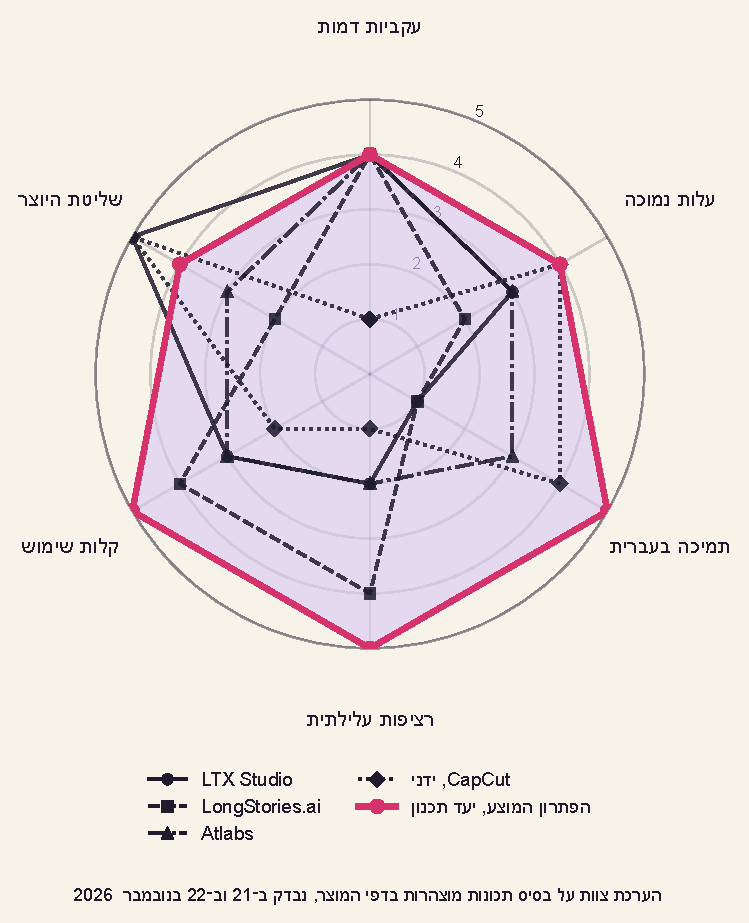
\includegraphics[width=0.8\textwidth]{figures/ch4_radar.pdf}
  \caption{תרשים רדאר: פרופיל ארבעה מתחרים ויעד התכנון. הערכת צוות על בסיס תכונות מוצהרות בדפי המוצר, נבדק ב־21.11.2026}
  \label{fig:ch4-radar}
\end{figure}

\subsection{גרף פיזור של יכולות מול עלות}
איור~\ref{fig:ch4-scatter} מעמת את מחיר התוכנית הזולה ביותר הכוללת דמויות עקביות עם מספר היכולות המרכזיות (מתוך ארבע) שבידי המוצר: דמויות עקביות, סדרה, עברית ווידאו מקצה לקצה. הגרף נועד להראות שאין מוצר בפינת הכיסוי המלא במחיר נמוך. נתוני עלות לדקת וידאו מוגמרת אינם זמינים, ולכן נבחרו ערכים שניתנים לאימות. יעד התכנון מסומן כיעד ולא כמוצר שנמדד.

\begin{figure}[h]
  \centering
  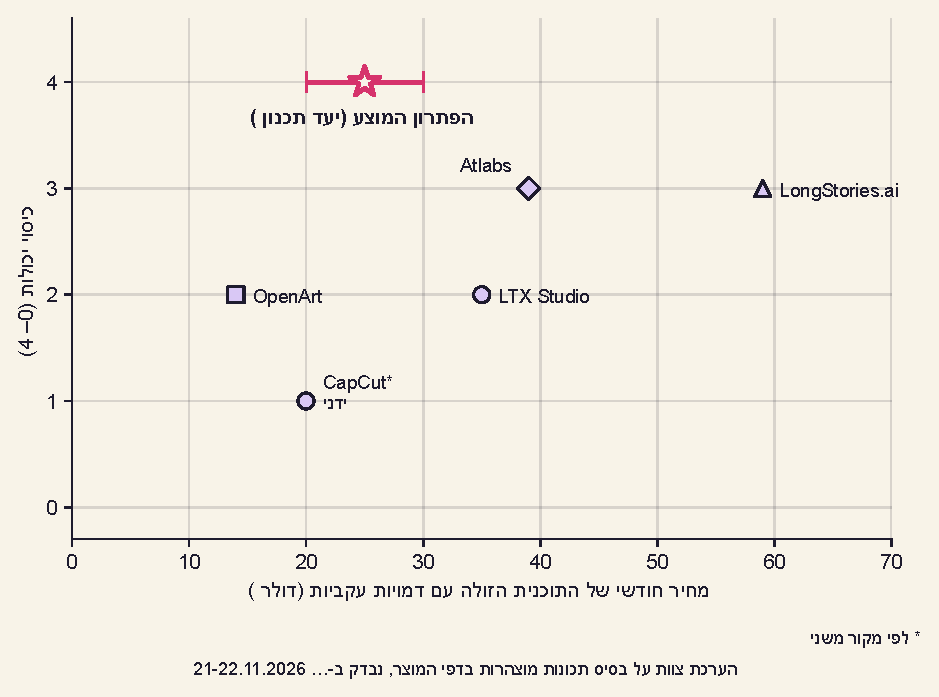
\includegraphics[width=0.8\textwidth]{figures/ch4_scatter.pdf}
  \caption{גרף פיזור: מחיר חודשי מול מספר יכולות מרכזיות. הערכת צוות על בסיס תכונות מוצהרות בדפי המוצר, נבדק ב־21.11.2026}
  \label{fig:ch4-scatter}
\end{figure}

\subsection{מגבלות הסקירה}
חלק מהכלים לא ניתנו לבדיקה ללא תשלום, ולכן ציוני קלות השימוש הם בחלקם הערכה. תמיכת \textenglish{Atlabs} בעברית מבוססת על התכתבות עם צוות התמיכה שלו ולא על בדיקה עצמאית. מחירי \textenglish{Atlabs} ו־\textenglish{CapCut} טרם אומתו מול דפי המחירים \textenglish{[TO-VERIFY]}, וכל הציונים בתרשים הרדאר הם שיפוט צוות. הסקירה אינה ממצה; קריטריוני בחירת חמשת המוצרים \textenglish{[TO-VERIFY]}, והנתונים הם תמונת מצב אחת מ־21.11.2026 שעשויה להשתנות.

\begin{directornote}
  בפרויקט שלנו הממצא המרכזי הוא שאף כלי לא נבדק בעברית בתוכנית חינמית, ולכן הפער הנגיש ליוצר דובר עברית נשאר פתוח. מחיר היעד של 20 עד 30 דולר נקבע כדי להימצא בטווח של המתחרים הזולים, ואומדני השוק הזמין והשוק היעד יעודכנו לאחר אימות ההנחות.
\end{directornote}
